% =============================================================================
% Tesis de maestría -- versión en ESPAÑOL
% Compilar:  tectonic main.tex   (o latexmk -pdf main.tex en Overleaf/TeXLive)
% =============================================================================
\documentclass[12pt, oneside]{report}

\usepackage[T1]{fontenc}
\usepackage[utf8]{inputenc}
\usepackage[spanish, es-tabla]{babel}

% =============================================================================
% Shared, language-neutral preamble.
% Each main.tex loads its documentclass + babel language FIRST, then \input's
% this file. Do NOT put \documentclass or babel here.
% =============================================================================

% --- Page geometry & spacing ---------------------------------------------------
\usepackage{geometry}
\geometry{a4paper, top=2.5cm, bottom=2.5cm, inner=3cm, outer=2.5cm}
\usepackage{setspace}
\onehalfspacing
\usepackage{microtype}

% --- Math ----------------------------------------------------------------------
\usepackage{amsmath, amssymb, mathtools}

% --- Graphics & figures --------------------------------------------------------
\usepackage{graphicx}
\graphicspath{{../common/figures/}{figures/}}
\usepackage{float}
\usepackage{caption}
\usepackage{subcaption}
\captionsetup{font=small, labelfont=bf}

% --- Tables --------------------------------------------------------------------
\usepackage{booktabs}
\usepackage{array}
\usepackage{tabularx}
\usepackage{longtable}
\usepackage{multirow}
\usepackage{siunitx}
\sisetup{group-separator={,}, group-minimum-digits=4, detect-weight=true, detect-family=true}

% --- Algorithms ----------------------------------------------------------------
\usepackage{algorithm}
\usepackage{algpseudocodex}

% --- Lists, color, misc --------------------------------------------------------
\usepackage{enumitem}
\usepackage{xcolor}
\definecolor{linknavy}{RGB}{20,60,110}

% --- Bibliography (biblatex + bibtex backend: compiles under tectonic; switch to
%     backend=biber on Overleaf for author-year/APA sorting if desired) ---------
\usepackage[backend=bibtex, style=ieee, sorting=nyt]{biblatex}
\addbibresource{../common/references.bib}

% --- Hyperlinks (load late) ----------------------------------------------------
\usepackage[hidelinks, breaklinks=true]{hyperref}
\hypersetup{colorlinks=true, linkcolor=linknavy, citecolor=linknavy, urlcolor=linknavy}
\usepackage[nameinlink]{cleveref}

% --- Project-specific shortcuts ------------------------------------------------
\newcommand{\ageb}{\textsc{ageb}\xspace}
\usepackage{xspace}
\renewcommand{\ageb}{\textsc{ageb}\xspace}
\newcommand{\nppv}{NPP--V\xspace}
\newcommand{\zmg}{ZMG\xspace}
\newcommand{\betadecay}{\ensuremath{\beta}}
\newcommand{\code}[1]{\texttt{#1}}

% Placeholder note for unfinished sections (visible but unobtrusive).
\newcommand{\todo}[1]{\medskip\noindent{\color{red!70!black}\small[\,TODO: #1\,]}\medskip}
\newcommand{\placeholder}{\todo{section to be written}}


% --- Metadatos de la tesis (editar) -------------------------------------------
\newcommand{\thesistitle}{Un marco transferible y orientado a la demanda para la
  priorización y generación de corredores de transporte público}
\newcommand{\thesissubtitle}{Análisis Nodo--Lugar--Personas de la Zona
  Metropolitana de Guadalajara}
\newcommand{\thesisauthor}{Alejandro Guevara}
\newcommand{\thesisadvisor}{[Nombre del director]}
\newcommand{\thesisprogram}{Maestría en [Programa]}
\newcommand{\thesisuniversity}{[Universidad]}
\newcommand{\thesisyear}{2026}

\begin{document}

% ---- Preliminares (numeración romana) ----
\pagenumbering{roman}
\begin{titlepage}
\centering
\vspace*{1cm}

{\scshape\Large \thesisuniversity \par}
\vspace{0.3cm}
{\large \thesisfaculty \par}
\vspace{0.5cm}
{\scshape \thesisprogram \par}
\vspace{2.5cm}

\rule{\linewidth}{0.4pt}\\[0.4cm]
{\huge\bfseries \thesistitle \par}
\vspace{0.4cm}
{\Large \thesissubtitle \par}
\rule{\linewidth}{0.4pt}\\[1.5cm]

{\Large\itshape \thesisauthor \par}
\vspace{2cm}

\begin{flushright}
\textit{Director de tesis:}\\
\thesisadvisor
\end{flushright}

\vfill
{\large Tesis presentada para obtener el grado de\\
\thesisprogram \par}
\vspace{1cm}
{\large \thesisyear \par}

\end{titlepage}
\clearpage

\chapter*{Resumen}
\addcontentsline{toc}{chapter}{Resumen}

Los enfoques convencionales basados en datos para la planeación del transporte
público con frecuencia predicen dónde el transporte \emph{ya existe} en lugar de
dónde se \emph{necesita}, produciendo modelos circulares que premian el statu quo.
Esta tesis desarrolla un marco transferible y orientado a la demanda que, en
cambio, diagnostica la demanda de transporte \emph{no atendida} y genera corredores
candidatos para atenderla, aplicado a la Zona Metropolitana de Guadalajara
(\zmg; \num{1881} áreas geoestadísticas básicas, \ageb, en diez municipios).

El marco se desarrolla en ocho etapas encadenadas: (i)~una superficie de demanda de
transporte estimada a partir de datos censales, económicos y de la red vial
mediante un modelo gravitacional doblemente restringido; (ii)~la calibración del
parámetro de decaimiento por distancia contra la Encuesta Origen--Destino 2022;
(iii)~una capa de oferta que mide la accesibilidad basada en \textsc{gtfs} y un
índice independiente de \emph{brecha de cobertura} que se convierte en la variable
objetivo supervisada, eliminando la circularidad de las etiquetas de ``tiene
parada''; (iv)~un mapa de priorización Nodo--Lugar--Personas con un término
explícito de equidad; (v)~una función formal de evaluación multiobjetivo; (vi)~un
generador de corredores basado en anclas de frontera, un tronco de diámetro sobre
el árbol de expansión mínima y una compuerta de factibilidad por rectitud;
(vii)~una auditoría de la red existente; y (viii)~un conjunto de validación que
combina retro-pruebas de exclusión, comparación y métricas de cobertura antes y
después.

La capa de diagnóstico es la contribución sólida: el índice de brecha de cobertura
se corrobora fuera de muestra con la apertura en 2025 de la Línea~4 de \zmg, cuyo
corredor presenta \num{1.6} veces la tasa metropolitana de brecha alta. La capa
generativa produce al menos un corredor sustantivo, factible y meritorio, a la vez
que caracteriza honestamente sus limitaciones. Finalmente, todo el marco se
transfiere de principio a fin a dos zonas metropolitanas de tamaño contrastante
---Toluca y Aguascalientes---, demostrando que es genuinamente portable y no un
desarrollo a la medida de \zmg.

\vspace{1em}
\noindent\textbf{Palabras clave:} transporte público; demanda de viajes; brecha de
cobertura; modelo Nodo--Lugar; optimización multiobjetivo; equidad; \textsc{gtfs};
transferibilidad; Guadalajara.

\clearpage

\chapter*{Agradecimientos}
\addcontentsline{toc}{chapter}{Agradecimientos}

\placeholder

\clearpage


\tableofcontents
\listoffigures
\listoftables
\clearpage

% ---- Cuerpo (numeración arábiga) ----
\pagenumbering{arabic}
\chapter{Introducción}
\label{ch:introduccion}

\section{Motivación}
% El reto de movilidad de la ZMG; dependencia del automóvil; el costo de una
% inversión mal asignada en transporte.
\placeholder

\section{El problema de circularidad en la planeación basada en datos}
% Los modelos que predicen dónde ya existe transporte ("tiene parada") premian el
% statu quo y no pueden identificar la necesidad no atendida.
\placeholder

\section{Preguntas de investigación}
\begin{description}
  \item[PI1 -- Demanda.] ¿Puede estimarse la demanda de transporte a resolución de
    \ageb solo a partir de datos de Nivel~1 (no de transporte)?
  \item[PI2 -- Diagnóstico.] ¿Un índice independiente de brecha de cobertura
    identifica zonas genuinamente desatendidas, y puede validarse fuera de muestra?
  \item[PI3 -- Generación.] ¿Pueden generarse y evaluarse corredores candidatos con
    base en necesidad genuina, no redundancia y eficiencia de demanda?
  \item[PI4 -- Transferibilidad.] ¿El marco se transfiere a otras zonas
    metropolitanas sin rediseño a la medida?
\end{description}

\section{Contribuciones}
\placeholder

\section{Estructura de la tesis}
% Un párrafo que mapea los capítulos a las ocho etapas.
\placeholder

\chapter{Marco Teórico y Trabajos Relacionados}
\label{ch:marco}

\section{El modelo Nodo--Lugar y sus extensiones}
% Modelo Nodo-Lugar de Bertolini; extensiones NP-RV / NPP-V.
\placeholder

\section{Estimación de la demanda de viajes}
% Modelo de cuatro pasos; modelos gravitacionales / de interacción espacial;
% balanceo doblemente restringido (Furness).
\placeholder

\section{Accesibilidad y análisis de brecha de cobertura}
% Accesibilidad de oportunidades acumuladas; desiertos de transporte.
\placeholder

\section{Análisis multicriterio y ponderación objetiva}
% CRITIC y método de entropía; equidad en la priorización.
\placeholder

\section{Aprendizaje automático para ubicación de estaciones y corredores}
% Random Forest / gradient boosting; interpretabilidad SHAP; riesgo de objetivo
% circular.
\placeholder

\section{Diseño de redes y generación de corredores}
% Heurísticas de árbol de Steiner; enfoques de árbol de expansión mínima.
\placeholder

\section{Vacío de investigación}
\placeholder

\chapter{Área de Estudio y Datos}
\label{ch:datos}

Este capítulo describe el área de estudio, la unidad espacial de análisis y los datos que
alimentan la metodología. Un tema recurrente es la integridad de los datos: varios de los
resultados de esta tesis dependen de correcciones a la geografía base y a indicadores
específicos que se descubrieron durante una reconstrucción completa de reproducibilidad, y
se documentan aquí para que las cifras de todo el trabajo sean rastreables.

\section{La Zona Metropolitana de Guadalajara}
\label{sec:datos-zmg}

El área de estudio principal es la Zona Metropolitana de Guadalajara (\zmg), la segunda
más grande de México. Siguiendo la delimitación oficial, comprende diez municipios del
estado de Jalisco, que abarcan un núcleo central denso (Guadalajara y Zapopan) y una
periferia en rápida urbanización (\cref{tab:municipios}). Su movilidad se caracteriza por
una dependencia del automóvil alta y creciente, un extenso sistema de autobuses
concesionado y de operación informal y, más recientemente, una pequeña capa prémium de
autobús de tránsito rápido (Mi Macro) y tren ligero (Mi Tren). Esta capa prémium sigue el
patrón latinoamericano más amplio en que el autobús de tránsito rápido se ha expandido con
rapidez como complemento costo-efectivo del ferrocarril
\parencite{hidalgo2013brt, cervero2013brt}; injertarlo sobre una red base mayormente
concesionada es justamente el contexto que motiva un enfoque de planeación basado en la
demanda en lugar de uno que sigue a la oferta.

\begin{table}[htbp]
\centering
\caption{Los diez municipios de la \zmg y su número de \ageb{}s.}
\label{tab:municipios}
\begin{tabular}{lS[table-format=3.0]}
\toprule
Municipio & {\ageb{}s} \\
\midrule
Zapopan                       & 481 \\
Guadalajara                   & 404 \\
Tlajomulco de Zúñiga          & 341 \\
San Pedro Tlaquepaque         & 213 \\
Tonalá                        & 207 \\
El Salto                      & 115 \\
Zapotlanejo                   & 41  \\
Ixtlahuacán de los Membrillos & 34  \\
Acatlán de Juárez             & 29  \\
Juanacatlán                   & 16  \\
\midrule
\textbf{Total}                & \textbf{1881} \\
\bottomrule
\end{tabular}
\end{table}

\section{El \ageb como unidad de análisis}
\label{sec:datos-ageb}

Todos los indicadores se agregan al \ageb (\emph{área geoestadística básica}), la unidad
de enumeración censal definida por el INEGI. El \ageb es lo bastante fino para resolver la
variación intraurbana en demanda y acceso, y a la vez lo bastante grueso para que los
atributos censales se reporten a su nivel. El universo de análisis se restringe a los
\ageb{}s urbanos de los diez municipios de la \zmg: se excluyen las celdas cuyo
\code{CVE\_AGEB} lleva un sufijo alfabético (\ageb{}s rurales), así como todos los
municipios fuera de la delimitación metropolitana. Tras este filtro el universo es de
\num{1881} \ageb{}s (\cref{tab:municipios}) ---y no los \num{2068} usados en versiones
previas de este trabajo, discrepancia que se explica en \cref{sec:datos-integridad}.

\section{Fuentes de datos}
\label{sec:datos-fuentes}

La metodología separa deliberadamente los datos de \emph{Nivel~1} ---censales, económicos
y de red, disponibles para cualquier ciudad mexicana--- de los datos de oferta de
transporte, usados únicamente para medir la brecha de cobertura y auditar las rutas
existentes. La \cref{tab:fuentes-datos} lista las fuentes principales.

\begin{table}[htbp]
\centering
\caption{Principales fuentes de datos y su papel en la metodología.}
\label{tab:fuentes-datos}
\begin{tabularx}{\linewidth}{llX}
\toprule
Fuente & Nivel & Papel \\
\midrule
INEGI CPV2020    & \ageb / manzana & Población, proporción joven, propiedad vehicular \\
DENUE            & establecimiento & Proxies de empleo y atracción de POI \\
OpenStreetMap    & red             & Intersecciones, densidad vial, grafo vial \\
GTFS             & parada / ruta   & Accesibilidad existente y auditoría \\
EOD 2022         & zona de encuesta & Calibración del modelo gravitacional \\
CONAPO / CONEVAL & \ageb           & Marginación y rezago social (equidad) \\
\bottomrule
\end{tabularx}
\end{table}

\begin{description}[leftmargin=1.4em, style=nextline]
  \item[Censo y sociodemografía (INEGI CPV2020).] El Censo de Población y Vivienda 2020
    \parencite{inegi_cpv2020} aporta la población, la proporción de población joven usada
    para amplificar la generación de viajes y la propiedad vehicular de los hogares
    (\code{VPH\_AUTOM} sobre \code{VIVPAR\_HAB}) usada para derivar la propensión al
    transporte.
  \item[Actividad económica (DENUE).] El Directorio Estadístico Nacional de Unidades
    Económicas \parencite{inegi_denue} provee la ubicación de establecimientos, agregada a
    empleo por \ageb y a densidades de puntos de interés y comercio que impulsan la
    atracción de viajes y las oportunidades de accesibilidad.
  \item[Red vial (OpenStreetMap).] El grafo vial y los indicadores de Nodo derivados
    (densidad de intersecciones y de calles) provienen de \textsc{osm}
    \parencite{openstreetmap}, extraídos para los diez municipios con \textsc{osmnx}
    \parencite{boeing2017osmnx}.
  \item[Oferta de transporte (GTFS).] La fuente \textsc{gtfs} de SITEUR define la red
    existente usada para la superficie de accesibilidad (\cref{sec:w3}) y la auditoría de
    rutas (\cref{sec:w7}).
  \item[Encuesta Origen--Destino (EOD 2022).] La encuesta metropolitana de viajes 2022
    \parencite{imeplan_eod2022} provee flujos zonales observados para calibrar el
    decaimiento con la distancia del modelo gravitacional (\cref{sec:w2}).
  \item[Índices de equidad (CONAPO, CONEVAL).] El índice de marginación
    \parencite{conapo_marginacion2020} y el índice de rezago social
    \parencite{coneval_rezago2020} conforman el término de equidad (\cref{eq:equity}).
\end{description}

\section{Convenciones espaciales e integridad de datos}
\label{sec:datos-integridad}

Todo el cómputo usa el sistema de referencia proyectado canónico EPSG:6372 (cónico
equidistante para México); las coordenadas geográficas (EPSG:4326) se usan solo para la
ingesta. Todas las columnas de geometría están indexadas espacialmente.

Una reconstrucción completa de reproducibilidad, desde cero, sacó a la luz tres defectos de
integridad silenciosamente presentes en versiones previas, todos ya corregidos. Primero, un
error de dedo en el código de municipio del filtro de la geografía base había eliminado un
municipio entero en cada reconstrucción; corregirlo, junto con excluir correctamente los
\ageb{}s de sufijo alfabético, da el universo de \num{1881} \ageb{}s usado en todo el
trabajo (las cifras anteriores, computadas contra una tabla de \num{2068} filas nunca
reproducible, deben leerse como superadas). Segundo, el ráster de elevación digital se había
cargado bajo una referencia espacial equivocada, produciendo valores de pendiente
geométricamente sin sentido; el modelo heredado afectado se retiró en lugar de re-ejecutarse.
Tercero, el índice de marginación entraba al término de equidad con el signo invertido y con
un relleno de ceros fuera de rango para los \ageb{}s no emparejados, lo que en conjunto había
permitido que el bono de equidad premiara a las zonas \emph{menos} marginadas; corregir la
dirección y usar imputación por mediana restaura un término de equidad monótono y con el
signo correcto. Estas correcciones afectan de manera sustantiva varias cifras principales y
son la razón por la que los resultados de esta tesis superan cualquier cifra anterior para
las mismas cantidades.

\chapter{Metodología}
\label{ch:metodologia}

Este capítulo presenta el marco orientado a la demanda en su totalidad. Se
organiza en ocho etapas encadenadas (\crefrange{sec:w1}{sec:w8}), resumidas en la
\cref{fig:pipeline}. El principio de diseño rector es una separación estricta entre
una capa de \emph{diagnóstico} (etapas W1--W4), que estima dónde se necesita el
transporte con independencia de dónde existe actualmente, y una capa
\emph{generativa y de validación} (W5--W8), que propone y evalúa corredores
candidatos. Todo el cómputo espacial se realiza en el sistema de referencia
proyectado canónico EPSG:6372, y todos los indicadores se agregan al \ageb, el área
geoestadística básica utilizada como unidad de análisis.

\begin{figure}[htbp]
  \centering
  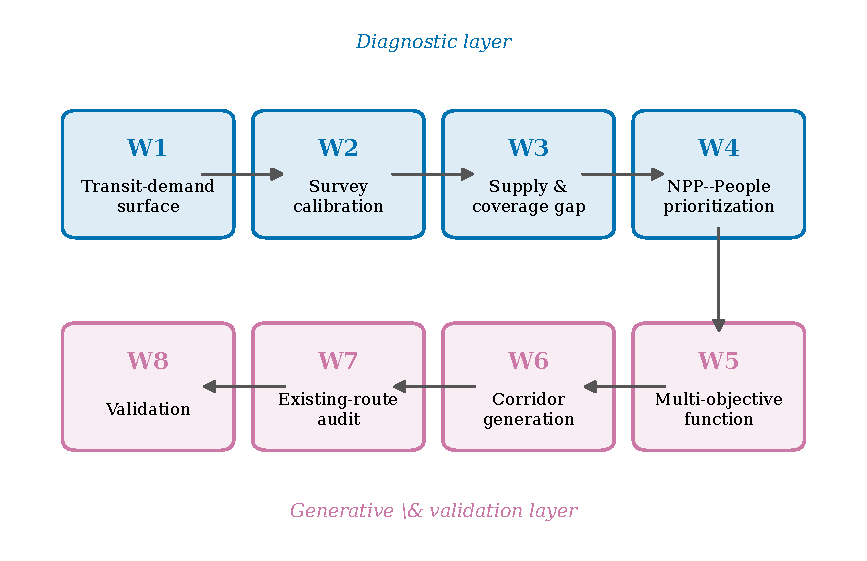
\includegraphics[width=\linewidth]{pipeline.pdf}
  \caption{El marco orientado a la demanda de ocho etapas. La capa de diagnóstico
    (W1--W4) está desacoplada de la oferta existente; la capa generativa y de
    validación (W5--W8) propone corredores y los pone a prueba.}
  \label{fig:pipeline}
\end{figure}

\section{Estimación de la demanda de transporte (W1)}
\label{sec:w1}

El marco inicia estimando una superficie de demanda de transporte a partir de datos
de \emph{Nivel~1} únicamente ---variables censales, económicas y de la red vial---,
excluyendo deliberadamente cualquier insumo de transporte existente, de modo que la
demanda nunca sea función de la oferta actual.

\subsection{Generación de viajes}
Las producciones diarias $P_i$ del \ageb $i$ se estiman a partir de la población con
una amplificación por proporción joven, que refleja las mayores tasas de viaje de
las cohortes jóvenes:
\begin{equation}
  P_i = \tau \, \mathrm{pob}_i \,\bigl(1 + \gamma\, s^{\text{joven}}_i\bigr),
  \label{eq:productions}
\end{equation}
con $\tau = \num{2.5}$ viajes por persona por día y $\gamma = \num{0.10}$. Las
atracciones combinan proxies de empleo y actividad,
\begin{equation}
  A_i = w_e\, e_i + w_p\, \rho^{\text{poi}}_i a_i + w_r\, \rho^{\text{comercio}}_i a_i,
  \label{eq:attractions}
\end{equation}
con $e_i$ el proxy de empleo, $\rho^{\text{poi}}_i$ y $\rho^{\text{comercio}}_i$ las
densidades de puntos de interés y comercio, y $a_i$ el área del \ageb. El vector de
atracción se escala luego para que $\sum_i A_i = \sum_i P_i$, condición necesaria
para el modelo doblemente restringido.

\subsection{Modelo gravitacional doblemente restringido}
Los flujos origen--destino $T_{ij}$ se obtienen de un modelo de interacción espacial
doblemente restringido \parencite{wilson1971gravity},
\begin{equation}
  T_{ij} = a_i\, b_j\, P_i\, A_j\, f(d_{ij}), \qquad
  f(d) = d^{-\beta},
  \label{eq:gravity}
\end{equation}
donde $f$ es una impedancia de ley de potencia sobre la distancia euclidiana entre
centroides $d_{ij}$ y $\beta$ es el parámetro de decaimiento por distancia
(calibrado en la \cref{sec:w2}). Los factores de balanceo $a_i,b_j$ imponen las
restricciones de producción y atracción,
\begin{equation}
  a_i = \Bigl(\textstyle\sum_j b_j A_j f(d_{ij})\Bigr)^{-1}, \qquad
  b_j = \Bigl(\textstyle\sum_i a_i P_i f(d_{ij})\Bigr)^{-1},
  \label{eq:furness}
\end{equation}
resueltos por ajuste proporcional iterativo (procedimiento de Furness), alternando
ambas actualizaciones hasta que los marginales convergen (tolerancia $10^{-5}$). Los
autoflujos se anulan en la diagonal y solo se conservan los pares con
$T_{ij}\ge\num{0.5}$ en la matriz dispersa de salida.

\subsection{Superficie de demanda de transporte}
La demanda total del \ageb $D_i = \tfrac12\sum_j (T_{ij}+T_{ji})$ se pondera
finalmente por un término de propensión al transporte derivado de la propiedad
vehicular de los hogares. Con
$v_i = \mathrm{VPH\_AUTOM}_i / \max(\mathrm{VIVPAR\_HAB}_i, 1)$ la tasa vehicular,
\begin{equation}
  D^{\text{transp}}_i = D_i \,(1 - v_i),
  \label{eq:transit-demand}
\end{equation}
de modo que las zonas con alta propiedad automovilística aportan proporcionalmente
menos demanda latente de transporte. La superficie resultante $D^{\text{transp}}$ es
la cantidad dependiente que impulsa el diagnóstico de brecha en la \cref{sec:w3}.

\section{Calibración con encuesta (W2)}
\label{sec:w2}

El parámetro de decaimiento $\beta$ se calibra contra la Encuesta Origen--Destino
2022 \parencite{imeplan_eod2022}. Los \ageb{}s se unen espacialmente a las zonas de
la encuesta, los flujos modelados se agregan a pares de zonas y se elige $\beta$
para minimizar la suma de errores al cuadrado en el espacio logarítmico entre los
flujos modelados y observados,
\begin{equation}
  \beta^\star = \arg\min_{\beta}\;
  \sum_{(z,z')} \Bigl(\log \hat{T}_{zz'}(\beta) - \log T^{\text{obs}}_{zz'}\Bigr)^2 .
  \label{eq:calibration}
\end{equation}
En el universo corregido de \num{1881} \ageb{}s esto arroja
$\beta^\star = \num{1.2005}$, que supera al prior inicial $\beta = \num{2.0}$ tanto
en RMSE como en $R^2$; el valor calibrado se adopta en todo el trabajo.

\section{Capa de oferta y brecha de cobertura (W3)}
\label{sec:w3}

\subsection{Accesibilidad al transporte}
La oferta existente se mide mediante una superficie de accesibilidad de
oportunidades acumuladas construida a partir del alimentador \textsc{gtfs}. Se
construye un grafo de transporte dirigido a partir de pares consecutivos de paradas;
desde cada \ageb se identifican las paradas de abordaje dentro de \SI{400}{\metre} y
una búsqueda de ruta más corta asigna a cada destino alcanzable un tiempo de viaje
generalizado
\begin{equation}
  t = t_{\text{cam}} + t_{\text{esp}} + t_{\text{veh}}
    = \frac{d_{\text{cam}}}{s_{\text{cam}}} + \frac{h}{2} + t_{\text{veh}},
  \label{eq:traveltime}
\end{equation}
con velocidad peatonal $s_{\text{cam}} = \SI{80}{\metre\per\minute}$ e intervalo
medio $h$. La accesibilidad es el empleo total alcanzable dentro de un presupuesto
de \SI{45}{\minute},
\begin{equation}
  \mathrm{Acc}_i = \sum_{j : t_{ij}\le 45} e_j .
  \label{eq:accessibility}
\end{equation}

\subsection{Índice de brecha de cobertura}
El diagnóstico central combina demanda y oferta en un índice de brecha de cobertura,
\begin{equation}
  g_i = \frac{D^{\text{transp}}_i}{\mathrm{Acc}_i + \varepsilon},
  \qquad \varepsilon = 1,
  \label{eq:gap}
\end{equation}
normalizado por una transformación $\log(1+x)$ seguida de un escalamiento min--máx
para dar $g^{\,n}_i \in [0,1]$. Los \ageb{}s se clasifican por quintiles conjuntos:
un \ageb es de \emph{brecha alta} cuando está en los dos quintiles superiores de
demanda y en los dos inferiores de accesibilidad, de \emph{brecha baja} en el caso
espejo y de \emph{brecha media} en el resto. La \cref{fig:coverage-gap} mapea el
resultado para \zmg.

\begin{figure}[htbp]
  \centering
  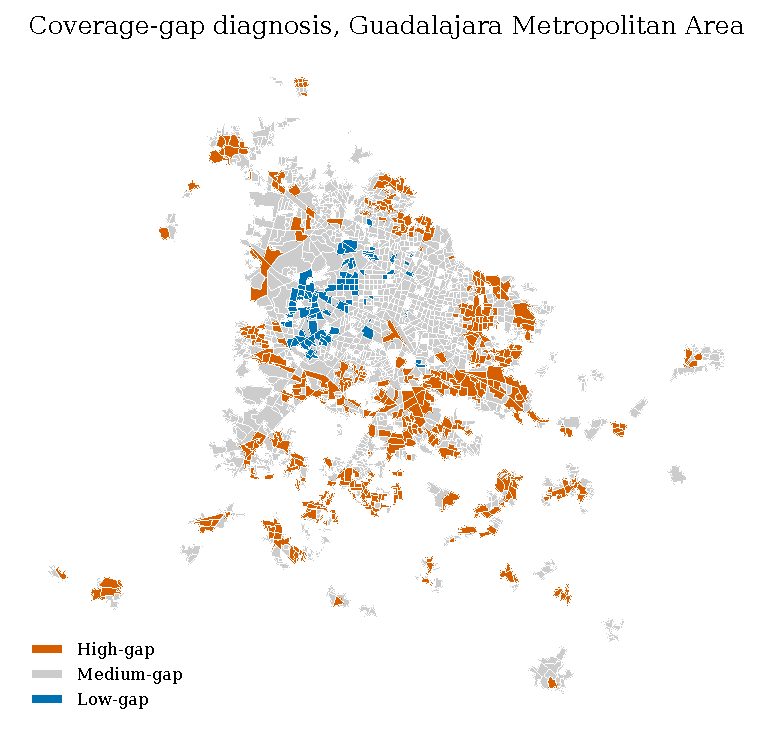
\includegraphics[width=0.82\linewidth]{zmg_coverage_gap.pdf}
  \caption{Diagnóstico de brecha de cobertura para la Zona Metropolitana de
    Guadalajara. El núcleo bien servido es de brecha baja; los \ageb{}s de brecha
    alta se concentran en la periferia.}
  \label{fig:coverage-gap}
\end{figure}

\subsection{Modelo supervisado sobre la brecha de cobertura}
Para interpretar los impulsores de la demanda no atendida, un objetivo binario
$y_i = \mathbb{1}[\text{categoría-}g_i = \text{brecha alta}]$ se regresa sobre los
\num{14} indicadores Nodo--Lugar--Personas (todas las variables de oferta excluidas
para evitar circularidad) mediante Random Forest y árboles potenciados por gradiente
\parencite{niu2023rf,ke2017lightgbm}. El comportamiento del modelo se interpreta con
valores SHAP \parencite{lundberg2017shap}; población, rezago social y empleo emergen
como los impulsores dominantes del estatus de brecha alta.

\section{Priorización Nodo--Lugar--Personas (W4)}
\label{sec:w4}

Con independencia de la demanda y la oferta, se calcula una puntuación de
priorización basada en el lugar a partir de los \num{14} indicadores normalizados.
Los pesos objetivos se derivan sin intervención de expertos combinando el método
CRITIC \parencite{diakoulaki1995critic} con el método de entropía. El peso CRITIC
del indicador $j$ premia tanto la dispersión como la independencia,
\begin{equation}
  w^{\text{c}}_j \propto \sigma_j \sum_{k} \bigl(1 - r_{jk}\bigr),
  \label{eq:critic}
\end{equation}
con $\sigma_j$ la desviación estándar del indicador $j$ y $r_{jk}$ su correlación
con el indicador $k$; ambas ponderaciones se promedian en un peso de ensamble $w_j$
(\cref{fig:weights}). La puntuación de lugar, el término de equidad y la puntuación
final son
\begin{align}
  \mathrm{NPP}_i &= \textstyle\sum_j w_j\, x^{\,n}_{ij}, \label{eq:npp}\\
  \mathrm{Eq}_i  &= \tfrac12\bigl(x^{\,n,\text{marg}}_i + x^{\,n,\text{rezago}}_i\bigr),
    \label{eq:equity}\\
  F_i &= (1-\alpha)\,\mathrm{NPP}_i + \alpha\,\mathrm{Eq}_i, \qquad \alpha = 0.20.
  \label{eq:final}
\end{align}
El término de equidad es un bono aditivo explícito y separable, de modo que las
puntuaciones pueden reportarse con y sin él; un análisis de sensibilidad sobre
$\alpha \in \{0.10, 0.20, 0.30\}$ confirma que el ordenamiento es robusto
(Spearman $\ge 0.98$).

\begin{figure}[htbp]
  \centering
  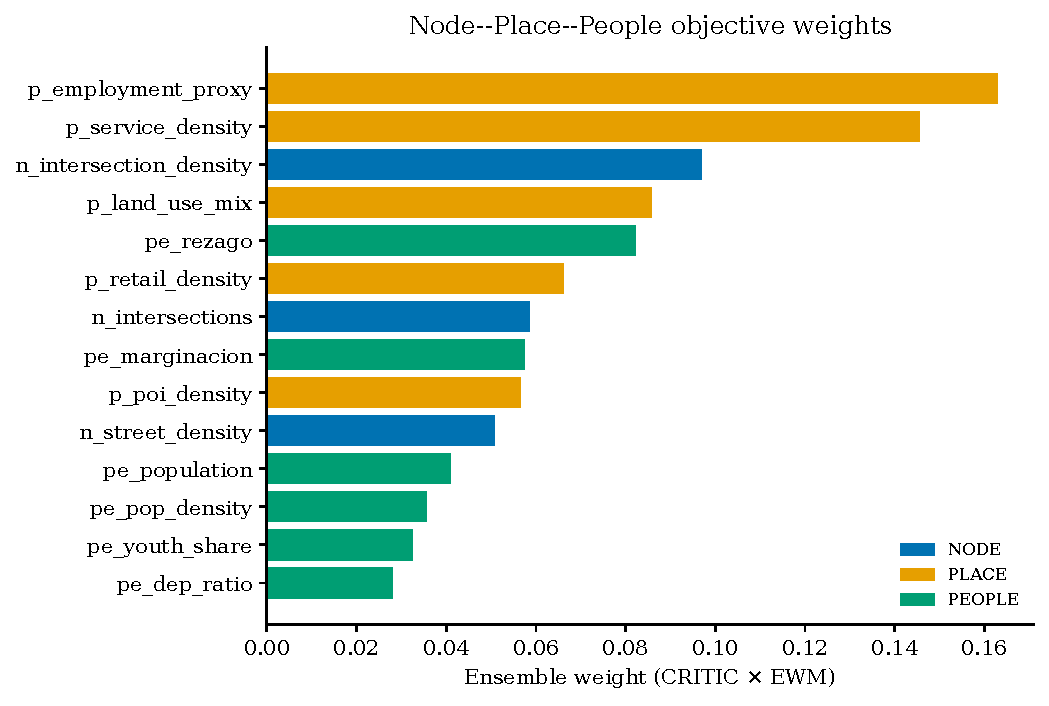
\includegraphics[width=0.85\linewidth]{w4_weights.pdf}
  \caption{Pesos objetivos de ensamble CRITIC$\,\times\,$EWM para los \num{14}
    indicadores Nodo--Lugar--Personas, coloreados por dimensión.}
  \label{fig:weights}
\end{figure}

\section{Función de evaluación multiobjetivo (W5)}
\label{sec:w5}

Los corredores candidatos (de W6) y las rutas existentes (en W7) se evalúan contra
tres objetivos en competencia: ganancia ponderada por demanda $f_1$ (maximizar),
longitud de ruta $f_2$ (minimizar) y equidad media $f_3$ (maximizar):
\begin{equation}
  f_1 = \frac{\sum_{i\in S} D_i\, \kappa\, u_i}{\sum_{i\in S} D_i}, \quad
  f_2 = \ell, \quad
  f_3 = \frac{1}{|S|}\sum_{i\in S}\mathrm{Eq}_i,
  \label{eq:objectives}
\end{equation}
donde $S$ es el conjunto de \ageb{}s servidos, $u_i = g^{\,n}_i$ la fracción no
atendida, $\ell$ la longitud de ruta y $\kappa$ un factor de ganancia ($\num{0.50}$
si el candidato conecta con la red existente, $\num{0.20}$ en otro caso). Un
candidato es \emph{factible} solo si satisface todas las restricciones:
\begin{equation}
  \frac{\ell}{\ell_{\text{tramo}}} \le 1.8, \quad
  \frac{\ell\cdot 10^3}{n_{\text{paradas}}-1} \in [300,1000]\,\si{\metre}, \quad
  \textstyle\sum_{i\in S} D_i \ge 500, \quad \ell \le \SI{30}{\kilo\metre},
  \label{eq:constraints}
\end{equation}
donde $\ell_{\text{tramo}}$ es el tramo en línea recta de las anclas del candidato
(el denominador de \emph{rectitud por anclas}; véase la \cref{sec:w6}). Los
candidatos se ordenan por clasificación no dominada (Pareto) minimizando
$(-f_1, f_2, -f_3)$.

\section{Generación de corredores (W6)}
\label{sec:w6}

Los corredores nuevos se generan con el \cref{alg:w6}. Los \ageb{}s de brecha alta
se restringen a la \emph{frontera} servido/no servido ---aquellos dentro de
\SI{400}{\metre} de la red existente--- para que los corredores generados conecten
intrínsecamente con ella. Las anclas de frontera se agrupan espacialmente; dentro de
cada grupo el corredor es la trayectoria hoja-a-hoja más larga (el \emph{tronco de
diámetro}) del árbol de expansión mínima de las anclas, ensamblada a partir de
segmentos reales de la red vial. La factibilidad usa la razón de rectitud por anclas
de la \cref{eq:constraints} en lugar de una razón de rodeo por extremos, porque esta
última penaliza en exceso a un corredor de cobertura de demanda que legítimamente se
curva. A cada corredor factible se le asigna un modo por umbral de demanda (tren
ligero $\ge \num{75000}$, autobús de tránsito rápido $\ge \num{15000}$, autobús
local en otro caso, viajes por día). La \cref{fig:corridors} muestra los cuatro
corredores factibles de \zmg.

\begin{algorithm}[htbp]
\caption{Generación de corredores por anclas de frontera (W6)}
\label{alg:w6}
\begin{algorithmic}[1]
\Require superficie de brecha $g^{\,n}$, demanda $D$, red vial $G$, paradas de la red
\State $H \gets$ clase Jenks superior de $g^{\,n}$ con $D \ge 500$
  \Comment{reserva de brecha alta}
\State $H \gets \{i \in H : \operatorname{dist}(i,\text{red}) \le \SI{400}{\metre}\}$
  \Comment{frontera}
\State particionar $H$ en $k$ grupos espaciales por $k$-medias
\ForAll{grupo $C$}
  \State $T \gets$ árbol de expansión mínima de $C$ sobre $G$
  \State $\pi \gets$ trayectoria hoja-a-hoja más larga de $T$ \Comment{tronco de diámetro}
  \State construir candidato desde $\pi$; evaluar $f_1,f_2,f_3$ y restricciones (W5)
\EndFor
\State \Return candidatos factibles, ordenados por Pareto
\end{algorithmic}
\end{algorithm}

\begin{figure}[htbp]
  \centering
  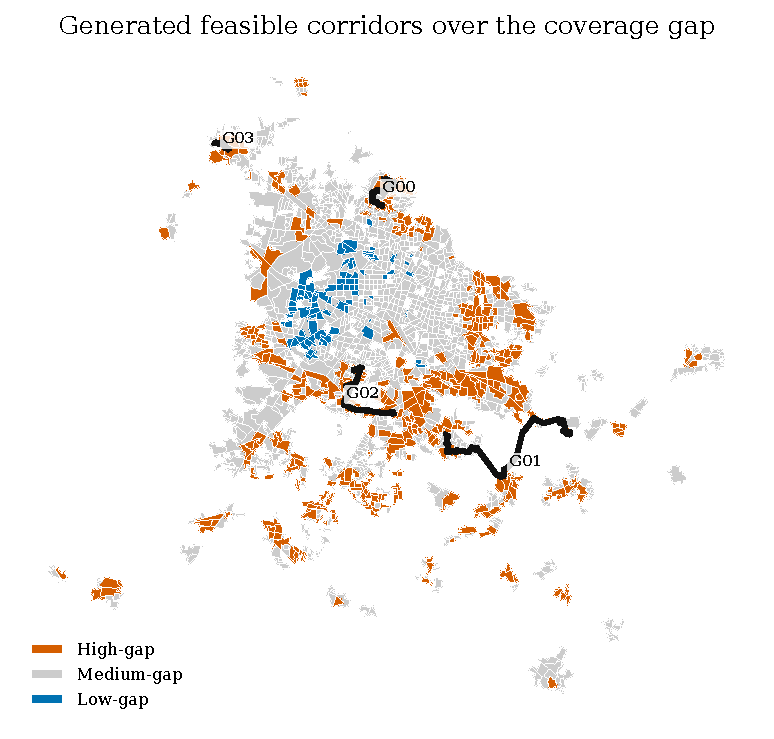
\includegraphics[width=0.82\linewidth]{zmg_corridors.pdf}
  \caption{Los cuatro corredores factibles generados (G00--G03) superpuestos sobre
    la superficie de brecha de cobertura.}
  \label{fig:corridors}
\end{figure}

\section{Auditoría de rutas existentes (W7)}
\label{sec:w7}

Cada ruta \textsc{gtfs} existente se evalúa con la misma función W5 y se marca como
\emph{baja demanda} ($f_1<\num{0.2}$ y puntuación total $<\num{0.3}$),
\emph{indirecta} (razón de rodeo $>\num{1.5}$) o \emph{redundante} (traslape de
Jaccard de \ageb{}s servidos $\ge\num{0.60}$ con una ruta de mayor puntuación). Las
rutas marcadas reciben una propuesta de modificación (atajo, fusión o retiro), lo
que hace la auditoría directamente comparable con los corredores generados.

\section{Validación (W8)}
\label{sec:w8}

El marco se valida de tres formas. Una \emph{retro-prueba de exclusión} enmascara el
nivel premium de transporte del alimentador \textsc{gtfs}, recalcula la accesibilidad
y la brecha de cobertura sin él, vuelve a ejecutar el generador y mide el traslape de
trazado entre los corredores re-propuestos y las rutas enmascaradas. Una
\emph{comparación} contrasta los corredores generados con las rutas premium
existentes. Finalmente, las \emph{métricas antes/después} ---tasa de cobertura,
coeficiente de Gini de la accesibilidad y población servida por kilómetro de ruta---
cuantifican la contribución marginal de los corredores generados. El
\cref{ch:resultados} reporta las tres para \zmg y el \cref{ch:transferibilidad} las
repite para las ciudades de transferencia.

\chapter{Resultados}
\label{ch:resultados}

Este capítulo reporta las salidas de cada etapa para la Zona Metropolitana de
Guadalajara (\zmg). El orden de las secciones sigue la metodología: la superficie de
demanda estimada (\cref{sec:res-w1}), su calibración (\cref{sec:res-w2}), el
diagnóstico de brecha de cobertura y su interpretación supervisada
(\cref{sec:res-w3}), la priorización Nodo--Lugar--Personas (\cref{sec:res-w4}), los
corredores generados (\cref{sec:res-w6}), la auditoría de la red existente
(\cref{sec:res-w7}) y el conjunto de validación (\cref{sec:res-w8}).

\section{Superficie de demanda de transporte estimada (W1)}
\label{sec:res-w1}

La metodología de Nivel~1 produce una estimación de demanda de transporte para los
\num{1881} \ageb{}s, con un total de \num{8471576} extremos de viaje en transporte al
día. La propiedad vehicular de los hogares varía ampliamente en la metrópoli: la tasa
vehicular media es \num{0.577}, lo que da una propensión media al transporte de
\num{0.423}. Como la demanda se pondera por $(1-v_i)$ (\cref{eq:transit-demand}), los
\ageb{}s con alta propiedad automovilística aportan proporcionalmente menos demanda
latente aun donde la generación bruta de viajes es alta. La \cref{fig:demand} mapea la
superficie resultante, que se concentra a lo largo de los densos corredores central y
oriente de la metrópoli.

\begin{figure}[htbp]
  \centering
  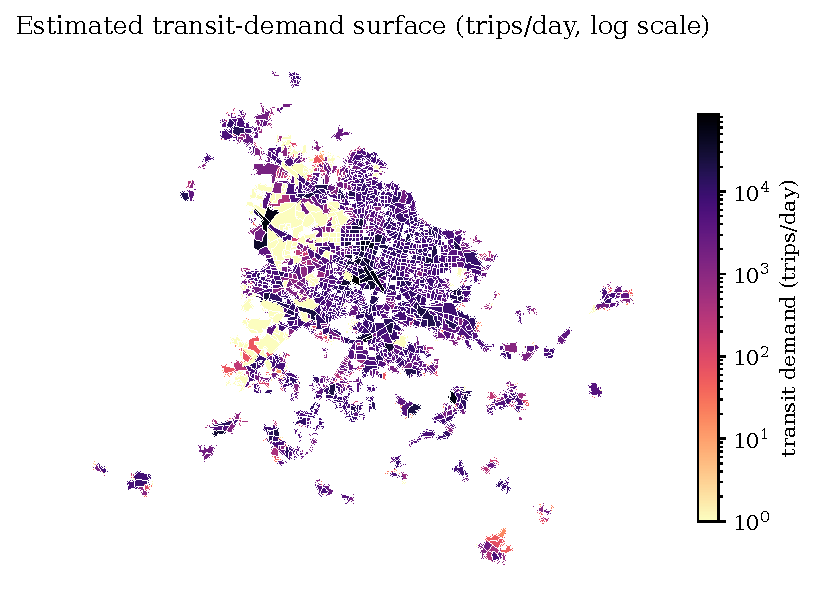
\includegraphics[width=0.82\linewidth]{zmg_demand.pdf}
  \caption{Superficie de demanda de transporte estimada (viajes por día por \ageb,
    escala logarítmica). La demanda se concentra en las zonas densas de menor
    propiedad vehicular del centro y el oriente.}
  \label{fig:demand}
\end{figure}

\section{Calibración del modelo gravitacional (W2)}
\label{sec:res-w2}

Calibrar el parámetro de decaimiento contra la Encuesta Origen--Destino 2022
(\cref{eq:calibration}) selecciona $\beta^\star = \num{1.2005}$, un decaimiento
notablemente más débil que el prior inicial $\beta = \num{2.0}$: los viajeros de \zmg
recorren distancias mayores de lo que suponía el prior. De manera crucial, el valor
calibrado \emph{mejora} el ajuste en el universo corregido de \num{1881} \ageb{}s en
todas las métricas (\cref{tab:calibration}), revirtiendo la conclusión provisional
obtenida sobre la tabla de \ageb{}s previa, mal filtrada. El $\beta$ calibrado se
adopta para la superficie de demanda y todas las etapas posteriores.

\begin{table}[htbp]
\centering
\caption{Calibración del modelo gravitacional contra la encuesta EOD 2022.}
\label{tab:calibration}
\begin{tabular}{lS[table-format=4.1]S[table-format=1.4]}
\toprule
Modelo & {RMSE (viajes)} & {$R^2$} \\
\midrule
Prior, $\beta = 2.0$        & 5088.2 & {--} \\
Calibrado, $\beta = 1.2005$ & 4524.9 & 0.2498 \\
\bottomrule
\end{tabular}
\end{table}

\section{Diagnóstico de brecha de cobertura (W3)}
\label{sec:res-w3}

La accesibilidad de oportunidades acumuladas (\cref{eq:accessibility}) combinada con
la superficie de demanda arroja el índice de brecha de cobertura (\cref{eq:gap}).
Clasificar los \ageb{}s por quintiles conjuntos de demanda/accesibilidad da
\num{390} de brecha alta (\SI{20.7}{\percent}), \num{1413} de brecha media y \num{78}
de brecha baja (\cref{tab:gap}). Como mostró la \cref{fig:coverage-gap}, las zonas de
brecha alta forman una periferia alrededor de un núcleo bien servido (brecha baja).

\begin{table}[htbp]
\centering
\caption{Clasificación de brecha de cobertura de los \num{1881} \ageb{}s de \zmg.}
\label{tab:gap}
\begin{tabular}{lS[table-format=4.0]S[table-format=2.1]}
\toprule
Categoría & {\ageb{}s} & {Proporción (\%)} \\
\midrule
Brecha alta  & 390  & 20.7 \\
Brecha media & 1413 & 75.1 \\
Brecha baja  & 78   & 4.1 \\
\bottomrule
\end{tabular}
\end{table}

Entrenar un modelo supervisado sobre el objetivo binario de brecha alta
(\cref{sec:w3}), con todas las variables de oferta excluidas, recupera bien la
estructura de la brecha y sin fuga de información (\cref{tab:retrain}). La atribución
SHAP ordena la población, el rezago social (\code{pe\_rezago}) y el proxy de empleo
como los impulsores dominantes: las zonas de brecha alta son áreas densas, de alta
necesidad y ricas en empleo que la red actual atiende de forma insuficiente.

\begin{table}[htbp]
\centering
\caption{Reentrenamiento supervisado sobre la brecha de cobertura (partición de prueba).}
\label{tab:retrain}
\begin{tabular}{lS[table-format=1.3]S[table-format=1.3]}
\toprule
Modelo & {PR-AUC} & {ROC-AUC} \\
\midrule
Random Forest & 0.877 & 0.962 \\
LightGBM      & 0.883 & 0.962 \\
\bottomrule
\end{tabular}
\end{table}

\section{Priorización Nodo--Lugar--Personas (W4)}
\label{sec:res-w4}

El procedimiento CRITIC$\,\times\,$EWM (\cref{eq:critic}) asigna los mayores pesos
objetivos al proxy de empleo (\num{0.163}), la densidad de servicios (\num{0.145}) y
la densidad de intersecciones de cuatro ramales (\num{0.097}); el vector completo de
pesos aparece en la \cref{fig:weights}. Promediada sobre todos los \ageb{}s, la
puntuación de lugar es $\overline{\mathrm{NPP}} = \num{0.4595}$, el término de
equidad $\overline{\mathrm{Eq}} = \num{0.2274}$ y el compuesto
$\overline{F} = \num{0.4131}$ con $\alpha = \num{0.20}$; la media baja de equidad es
esperada, ya que \zmg es predominantemente de baja marginación. Un análisis de
sensibilidad sobre $\alpha \in \{0.10, 0.20, 0.30\}$ confirma que la priorización es
robusta: el ordenamiento correlaciona con la línea base de $\alpha = \num{0.20}$ en
Spearman $\ge \num{0.98}$, de modo que el peso de equidad cambia cuáles \ageb{}s
específicos encabezan la lista sin alterar la estructura general.

\section{Corredores generados (W6)}
\label{sec:res-w6}

El generador produce cinco corredores candidatos, de los cuales cuatro son factibles
(\cref{tab:corridors}); el quinto (\code{W6\_G05}) se rechaza por la restricción de
rectitud por anclas (\num{1.93} > \num{1.8}). La \cref{fig:corridors} mapea los cuatro
corredores factibles sobre la superficie de brecha, y la \cref{fig:pareto} sitúa a
todos los candidatos en el espacio de objetivos.

\begin{table}[htbp]
\centering
\caption{Corredores candidatos generados. \code{W6\_G05} incumple la restricción de
  rectitud por anclas.}
\label{tab:corridors}
\begin{tabular}{l S[table-format=2.1] S[table-format=2.0] S[table-format=6.0] l c}
\toprule
Corredor & {km} & {\ageb{}s} & {Demanda/día} & Modo & Factible \\
\midrule
W6\_G00 & 7.3  & 18 & 66041  & BRT         & Sí \\
W6\_G01 & 23.0 & 27 & 96839  & Tren ligero & Sí \\
W6\_G02 & 12.1 & 25 & 192357 & Tren ligero & Sí \\
W6\_G03 & 2.4  & 5  & 35784  & BRT         & Sí \\
W6\_G05 & 5.4  & 14 & 80234  & Tren ligero & {--} \\
\bottomrule
\end{tabular}
\end{table}

\begin{figure}[htbp]
  \centering
  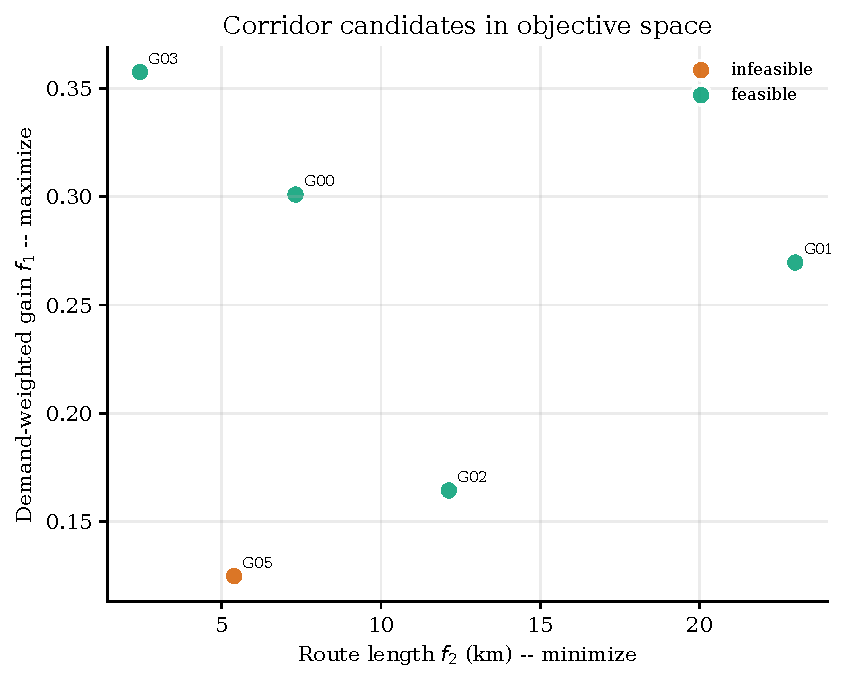
\includegraphics[width=0.78\linewidth]{w6_pareto.pdf}
  \caption{Corredores candidatos en el espacio de objetivos $(f_2, f_1)$, coloreados
    por factibilidad. Los corredores factibles cubren un rango de compromisos
    longitud/ganancia.}
  \label{fig:pareto}
\end{figure}

El resultado más destacado es \code{W6\_G02}: un corredor sustantivo de
\SI{12.1}{\kilo\metre} y \num{25} \ageb{}s que transporta una estimación de
\num{192357} viajes/día. En las pruebas de mérito introducidas para la validación
(\cref{sec:res-w8}) es el único corredor factible que pasa las tres: el
\SI{56}{\percent} de sus \ageb{}s servidos son de brecha alta (frente a la línea base
metropolitana de \SI{20.7}{\percent}), no es redundante con las rutas existentes
(mejor Jaccard \num{0.18}) y su demanda por kilómetro se ubica en el percentil
\num{73} de la red existente. \code{W6\_G03} también pasa, pero es un tramo corto de
\SI{2.4}{\kilo\metre}, mientras que \code{W6\_G00} y \code{W6\_G01} atienden necesidad
real pero son conectores de menor eficiencia ---un resultado mixto pero caracterizado
honestamente que se discute en el \cref{ch:discusion}.

\section{Auditoría de rutas existentes (W7)}
\label{sec:res-w7}

Evaluar las \num{247} rutas existentes de SITEUR con la misma función multiobjetivo
marca \num{229} de ellas (\cref{tab:audit}): \num{109} como indirectas, \num{80} como
de baja demanda y \num{40} como redundantes, dejando solo \num{18} sin marcar. La
\cref{fig:w7audit} grafica cada ruta en el espacio de objetivos por marca. Cada ruta
marcada lleva una propuesta de modificación (atajo, fusión o retiro), lo que hace la
auditoría directamente comparable con los corredores generados.

\begin{table}[htbp]
\centering
\caption{Marcas de auditoría en las \num{247} rutas existentes de SITEUR.}
\label{tab:audit}
\begin{tabular}{lS[table-format=3.0]}
\toprule
Marca & {Rutas} \\
\midrule
Indirecta    & 109 \\
Baja demanda & 80 \\
Redundante   & 40 \\
Sin marcar   & 18 \\
\bottomrule
\end{tabular}
\end{table}

\begin{figure}[htbp]
  \centering
  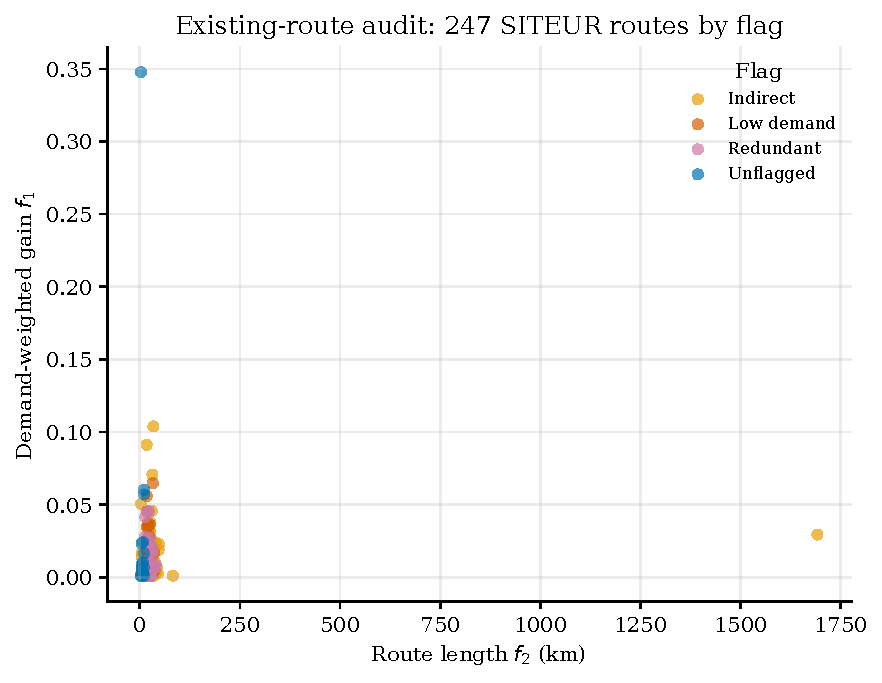
\includegraphics[width=0.82\linewidth]{w7_audit.pdf}
  \caption{Auditoría de rutas existentes: las \num{247} rutas de SITEUR en el espacio
    $(f_2, f_1)$, coloreadas por marca de auditoría.}
  \label{fig:w7audit}
\end{figure}

\section{Validación (W8)}
\label{sec:res-w8}

\paragraph{Retro-prueba de exclusión y comparación.} Enmascarar el nivel premium (Mi
Macro y Mi Tren) y volver a ejecutar el generador reproduce las rutas enmascaradas con
un traslape medio de trazado de apenas \SI{15.0}{\percent}; enmascarar líneas férreas
individuales da \SI{0}{\percent}. La comparación contra \num{33} rutas premium
existentes da un traslape medio de \SI{10.5}{\percent} para \SI{44.9}{\kilo\metre} de
corredor generado. El traslape bajo es el resultado esperado y deseado: el generador
identifica zonas genuinamente desatendidas en lugar de replicar líneas existentes. La
reconstrucción es, en todo caso, un proxy débil del mérito de un corredor
(\cref{ch:discusion}).

\paragraph{Métricas antes/después.} Agregar los corredores factibles a la red
existente mejora todas las métricas de cobertura (\cref{tab:beforeafter}): la tasa de
cobertura de \ageb{}s sube \num{1.1} puntos porcentuales, el Gini de accesibilidad cae
\num{0.0187} y \num{47} \ageb{}s antes desatendidos ---hogar de \num{120648}
personas--- ganan servicio.

\begin{table}[htbp]
\centering
\caption{Métricas de cobertura antes/después para los corredores W6 factibles.}
\label{tab:beforeafter}
\begin{tabular}{lS[table-format=2.1]S[table-format=2.1]S[table-format=+1.4]}
\toprule
Métrica & {Antes} & {Después} & {$\Delta$} \\
\midrule
Tasa de cobertura (\%) & 69.9   & 71.0   & +1.1 \\
Gini de accesibilidad  & 0.6333 & 0.6146 & -0.0187 \\
\bottomrule
\end{tabular}
\end{table}

\paragraph{Corroboración fuera de muestra.} La validación más fuerte es externa: la
instantánea \textsc{gtfs} de 2024 es anterior a la apertura en diciembre de 2025 de la
Línea~4 de SITEUR, por lo que el diagnóstico trata el corredor de la Línea~4 como
desatendido. Sus \ageb{}s muestran \num{1.6} veces la tasa metropolitana de brecha
alta, confirmando fuera de muestra que el índice de brecha de cobertura señala
corredores que los planificadores decidieron construir de forma independiente. Esto
corrobora la capa de \emph{diagnóstico}; no prueba que el generador hubiera producido
la Línea~4, distinción que se desarrolla en el \cref{ch:discusion}.

\chapter{Transferibilidad}
\label{ch:transferibilidad}

\section{Diseño del estudio}
% Dos metrópolis contrastantes: Toluca (grande) y Aguascalientes (compacta).
\placeholder

\section{Transferencia de demanda y brecha de cobertura}
% Gradiente de dependencia del automóvil; brecha alta ZMG 20.7\% > Toluca 14.9\%
% > Ags 9.6\%.
\placeholder

\section{Transferencia de priorización y generación de corredores}
% Los pesos se rederivan por ciudad; corredores factibles sustantivos en ambas.
\placeholder

\section{Transferencia de la validación}
% Auditoría W7; comparación W8 (traslape alto = re-identificación); retro-prueba de
% colapso de frontera.
\placeholder

\section{Error de transferencia y limitaciones}
\placeholder

\chapter{Discusión}
\label{ch:discusion}

\section{La capa de diagnóstico como contribución sólida}
% Corroboración fuera de muestra (Línea 4 a 1.6x la tasa metropolitana de brecha
% alta).
\placeholder

\section{La capa generativa: un éxito parcial y caracterizado}
% W6\_G02 pasa el mérito; persisten conectores de baja eficiencia; sin
% reconstrucción de líneas férreas.
\placeholder

\section{La reconstrucción es un proxy débil del mérito de un corredor}
% Por qué las retro-pruebas corroboran pero no prueban optimalidad.
\placeholder

\section{Implicaciones de equidad}
\placeholder

\section{Limitaciones}
\placeholder

\chapter{Conclusiones y Trabajo Futuro}
\label{ch:conclusiones}

\section{Síntesis de hallazgos}
\label{sec:concl-sintesis}

Esta tesis se propuso romper la circularidad que socava la planeación de transporte
basada en datos y construir, en su lugar, una metodología basada en la demanda que
diagnostica la necesidad no atendida, genera corredores candidatos y se transfiere a
otras ciudades. Las cuatro preguntas de investigación pueden responderse ahora de forma
directa.

\paragraph{PI1 -- Demanda.} \emph{Sí.} La demanda de transporte puede estimarse a
resolución de \ageb solo a partir de datos de Nivel~1. La generación de viajes y el modelo
gravitacional doblemente restringido del \cref{sec:w1} producen una superficie de demanda
metropolitana usando únicamente variables censales, económicas y de red, sin ningún insumo
de transporte, y la calibración contra la encuesta EOD~2022 (\cref{sec:w2}) fija el
parámetro de decaimiento en $\betadecay=1.2005$ ---un valor que ajusta los flujos
observados mejor que el previo convencional. La demanda, por tanto, nunca es función de la
oferta actual, que es la precondición de la que depende el resto del marco.

\paragraph{PI2 -- Diagnóstico.} \emph{Sí, y se valida fuera de muestra.} El índice de
brecha de cobertura (\cref{sec:w3}) contrapone la demanda modelada con la accesibilidad
medida por \textsc{gtfs}, produciendo una variable dependiente construida con independencia
de la oferta; el reentrenamiento supervisado la aprende de las características de lugar sin
fuga (\cref{tab:retrain}). Su mayor respaldo es el experimento natural de la Línea~4: un
corredor que el modelo nunca vio, luego elegido para construcción, muestra \num{1.6} veces
la tasa metropolitana de brecha alta. Este diagnóstico es la contribución más firme y
citable de la tesis.

\paragraph{PI3 -- Generación.} \emph{Parcialmente, y ahora caracterizada.} Una vez que los
corredores se modelan como trayectorias reales (un tronco por diámetro del árbol de
expansión mínima sobre el grafo vial) y se juzgan por rectitud respecto a las anclas en vez
de por el rodeo entre extremos (\cref{sec:w6}), el generador produce al menos un corredor
sustantivo, factible y que aprueba en mérito ---\code{W6\_G02}, \SI{12.1}{\kilo\metre},
\SI{56}{\percent} de brecha alta, no redundante, eficiencia de demanda en el percentil
\num{73}. También arroja conectores de menor eficiencia junto a él, y no reconstruye las
líneas férreas ya construidas ---un resultado esperado, pues la reconstrucción es un proxy
débil del mérito (\cref{sec:disc-reconstruction}). La capa generativa es así una
contribución genuina pero acotada.

\paragraph{PI4 -- Transferibilidad.} \emph{Sí, de extremo a extremo.} La metodología
completa W1--W8 corre sin rediseño a la medida en dos zonas metropolitanas contrastantes
---Toluca (grande, dieciséis municipios) y Aguascalientes (compacta, tres)---
re-derivando demanda, diagnóstico, pesos, corredores y auditoría a partir de los datos de
Nivel~1 y \textsc{gtfs} propios de cada ciudad (\cref{ch:transferibilidad}). El diagnóstico
diferencia sensatamente a las tres metrópolis por su proporción de demanda no atendida, y
la ponderación de cada ciudad se re-deriva de sus propios datos en lugar de heredar la de
la \zmg.

\section{Recomendaciones prácticas}
\label{sec:concl-recomendaciones}

Para una agencia de planeación, el marco es más útil como \emph{tamiz diagnóstico} que como
piloto automático. De ahí se siguen tres recomendaciones. Primera, tratar la superficie de
brecha de cobertura como el producto principal: ordena dónde se concentra la demanda no
atendida a una resolución más fina que cualquier línea individual, y puede recalcularse a
bajo costo conforme se actualizan los datos censales y \textsc{gtfs}. Segunda, usar la
auditoría de rutas (\cref{sec:w7}) para marcar rutas existentes de baja demanda, indirectas
y redundantes para su revisión ---en las ciudades de transferencia sacó a la luz una
redundancia sustancial de servicio paralelo, candidata a racionalización. Tercera, leer los
corredores generados como \emph{hipótesis a estudiar}, no como trazos finales: el corredor
que aprueba en mérito es un punto de partida defendible para un estudio de factibilidad,
pero las limitaciones caracterizadas del generador implican que su salida debe informar, no
reemplazar, el proceso de ingeniería y comunidad.

\section{Trabajo futuro}
\label{sec:concl-futuro}

Cuatro direcciones fortalecerían más el marco. Primera, la \emph{calibración local para las
ciudades de transferencia}: Toluca y Aguascalientes heredan hoy el previo de decaimiento de
la \zmg, y un $\betadecay$ calibrado con encuesta por ciudad afinaría sus superficies de
demanda. Segunda, un \emph{modelo gravitacional con distancia de red}: reemplazar la
impedancia euclidiana por impedancia de tiempo de viaje sobre el grafo vial mejoraría las
magnitudes absolutas de demanda. Tercera, \emph{transferir la capa supervisada}: el
reentrenamiento de brecha de cobertura se corrió solo para la \zmg, y aplicarlo a las
ciudades de transferencia probaría si la relación aprendida entre características de lugar y
demanda no atendida es en sí misma portable. Cuarta, un \emph{modelador híbrido de
corredores} que alterne entre el tronco por diámetro y el ruteo tipo agente viajero donde
este último siga siendo factible, lo que el análisis exploratorio sugiere que mejoraría
marginalmente la cobertura sin sacrificar factibilidad. Más allá de estas, la validación
externa más clara vendría de la afluencia observada en cualquier corredor que llegue a
construirse a lo largo de un trazo generado ---el contrafactual que, por construcción,
ningún estudio puramente ex ante puede aportar.


% ---- Material final ----
\printbibliography[heading=bibintoc]

\appendix
\chapter{Material Suplementario}
\label{app:suplementario}

\section{Definición de los indicadores NPP--V}
% Tabla completa de los 14 indicadores Nodo/Lugar/Personas y reglas de
% normalización.
\placeholder

\section{Reproducibilidad}
% Estructura del repositorio, orquestadores por etapa, configuración del entorno.
\placeholder


\end{document}
